\newpage
\section{Part A}

Part A is to write a MIPS assembly program for displaying the lowest 8
digits of my student ID on the DE2 board seven segment display \cite{ref:assignment_brief}.

Below is a program in MIPS assembly displays 01601082 on the DE2 board seven segment display.

\begin{minted}[
   fontsize=\footnotesize,
   linenos,
   breaklines,
]{MIPS}
.text
.globl _main
_main:
	# Construct the HEX0_R reg addr in GPR 1
	lui $t1, 0xFFFF  # Upper half addr
	ori $t1, $t1, 0x2010  # Lower half addr

	# Clear the upper 16 bits of GPR 0
	lui $t0, 0x0000

	# Set the lower 16 bits of GPR 0
	ori $t0, $zero, 0x0024  # decimal 2
	sw $t0, 0x0000($t1)  # Store the decimal 0 into the HEX0_R reg

	ori $t0, $zero, 0x0000  # decimal 8
	sw $t0, 0x0004($t1)  # Store the decimal 1 into the HEX1_R reg

	ori $t0, $zero, 0x0040  # decimal 0
	sw $t0, 0x0008($t1)  # Store the decimal 6 into the HEX2_R reg

	ori $t0, $zero, 0x0079  # decimal 1
	sw $t0, 0x000C($t1)  # Store the decimal 0 into the HEX3_R reg

	ori $t0, $zero, 0x0040  # decimal 0
	sw $t0, 0x0010($t1)  # Store the decimal 1 into the HEX4_R reg

	ori $t0, $zero, 0x0002  # decimal 6
	sw $t0, 0x0014($t1)  # Store the decimal 0 into the HEX5_R reg

	ori $t0, $zero, 0x0079  # decimal 1
	sw $t0, 0x0018($t1)  # Store the decimal 8 into the HEX6_R reg

	ori $t0, $zero, 0x0040  # decimal 0
	sw $t0, 0x002C($t1)  # Store the decimal 2 into the HEX7_R reg
\end{minted}

The code above were work as expect, as shown in Figure \ref{fig:part_a}

\begin{figure}[htbp]
   \centering
   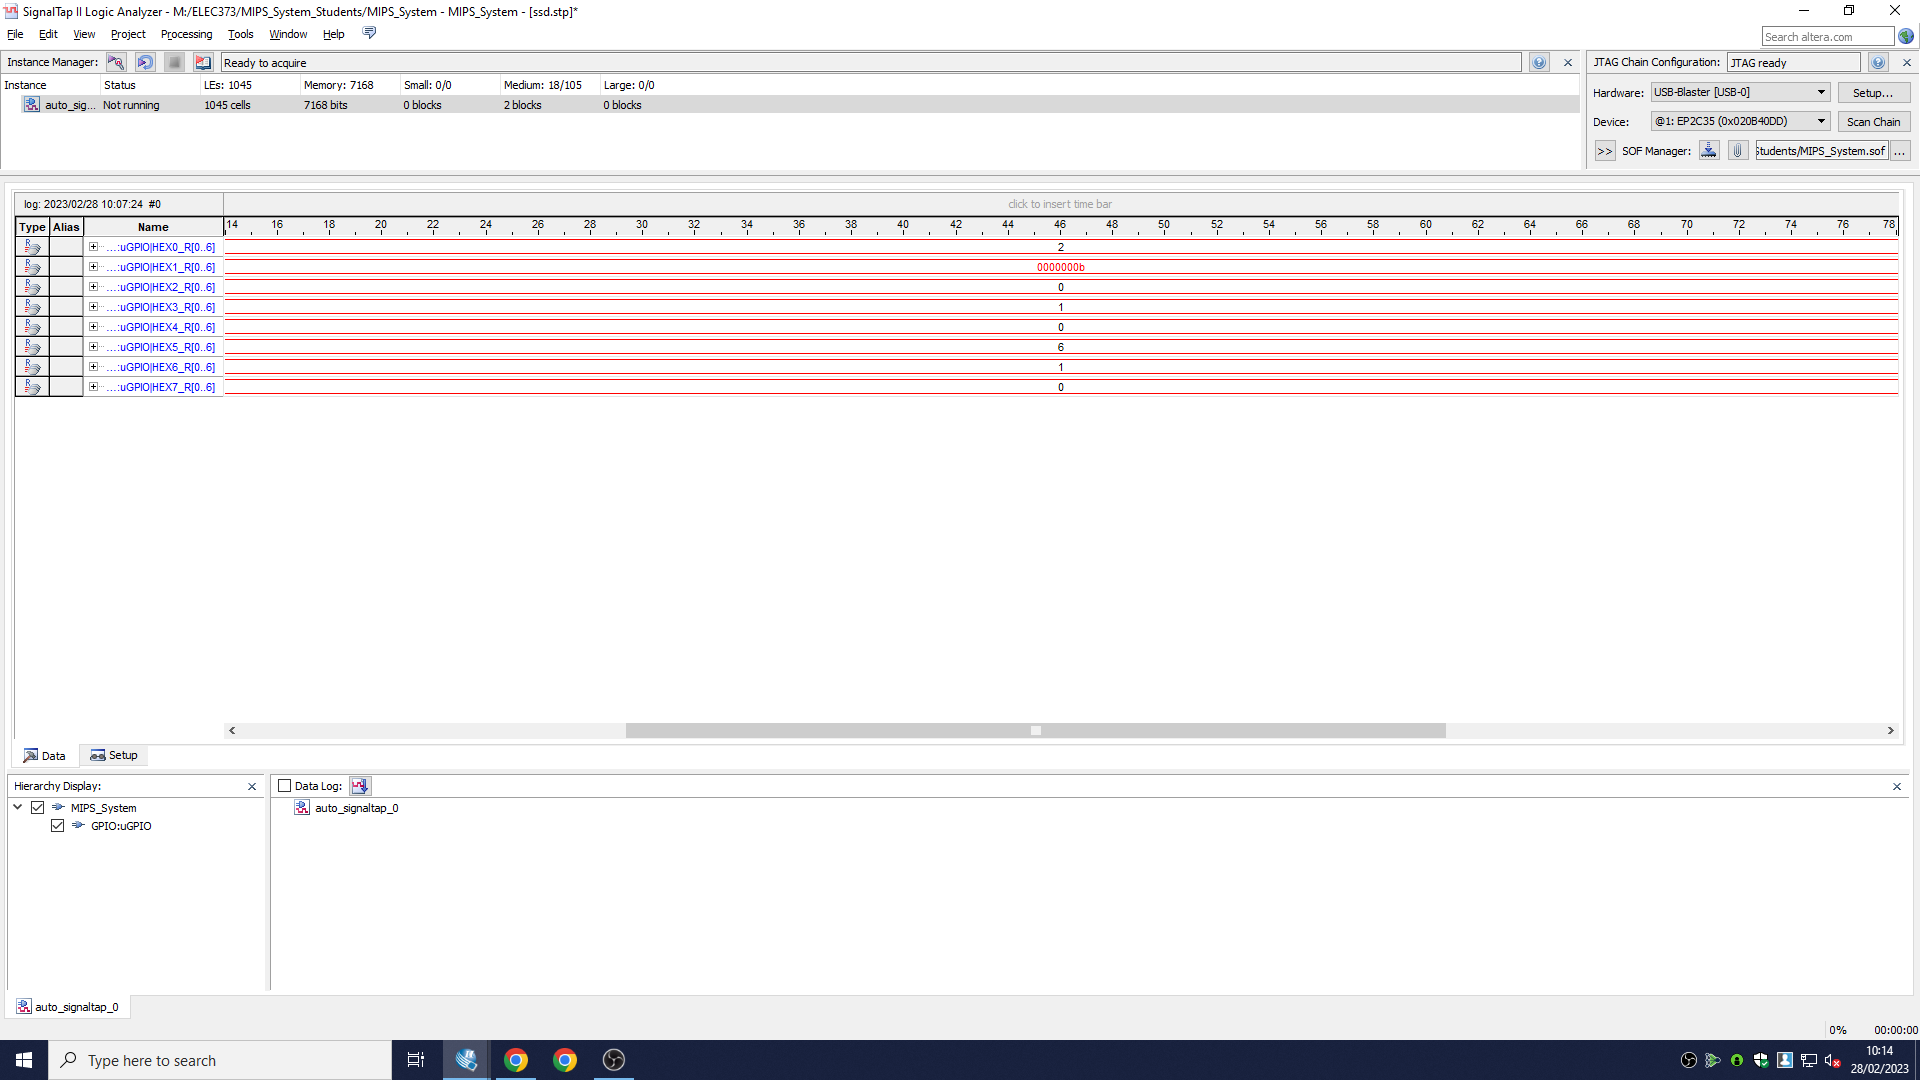
\includegraphics[width=\textwidth]{part_a}
   \caption{Result of Part A visualised by SignalTap. 0000000b is effectively 8 on the DE2 seven segment display.}
   \label{fig:part_a}
\end{figure}

\newpage
\subsubsection{Using data segment}

The code below is an attempt to simplify by using a \textit{.data} section. However, I didn't figure out how to use the dump of the \textit{.data} with the given MIPS implementation. Figure \ref{fig:dump} is the dumped data segment visualised in the \textit{MARS} editor.

\begin{minted}[
   fontsize=\footnotesize,
   linenos,
   breaklines,
]{MIPS}
.data
.word
first_ld: 18     # 2
second_ld: 0     # 8
third_ld: 64     # 0
fourth_ld: 121   # 1
fifth_ld: 64     # 0
sixth_ld: 2      # 6
seventh_ld: 121  # 1
eighth_ld: 64    # 0
HEX7_R: 0xFFFF202C
HEX6_R: 0xFFFF2028
HEX5_R: 0xFFFF2024
HEX4_R: 0xFFFF2020
HEX3_R: 0xFFFF201C
HEX2_R: 0xFFFF2018
HEX1_R: 0xFFFF2014
HEX0_R: 0xFFFF2010

.text
.globl _main
_main:
	lw $t0, first_ld
	sw $t0, HEX7_R

	lw $t0, second_ld
	sw $t0, HEX6_R

	lw $t0, third_ld
	sw $t0, HEX5_R

	lw $t0, fourth_ld
	sw $t0, HEX4_R

	lw $t0, fifth_ld
	sw $t0, HEX3_R

	lw $t0, sixth_ld
	sw $t0, HEX2_R

	lw $t0, seventh_ld
	sw $t0, HEX1_R

	lw $t0, eighth_ld
	sw $t0, HEX0_R
\end{minted}

\begin{figure}[htbp]
   \centering
   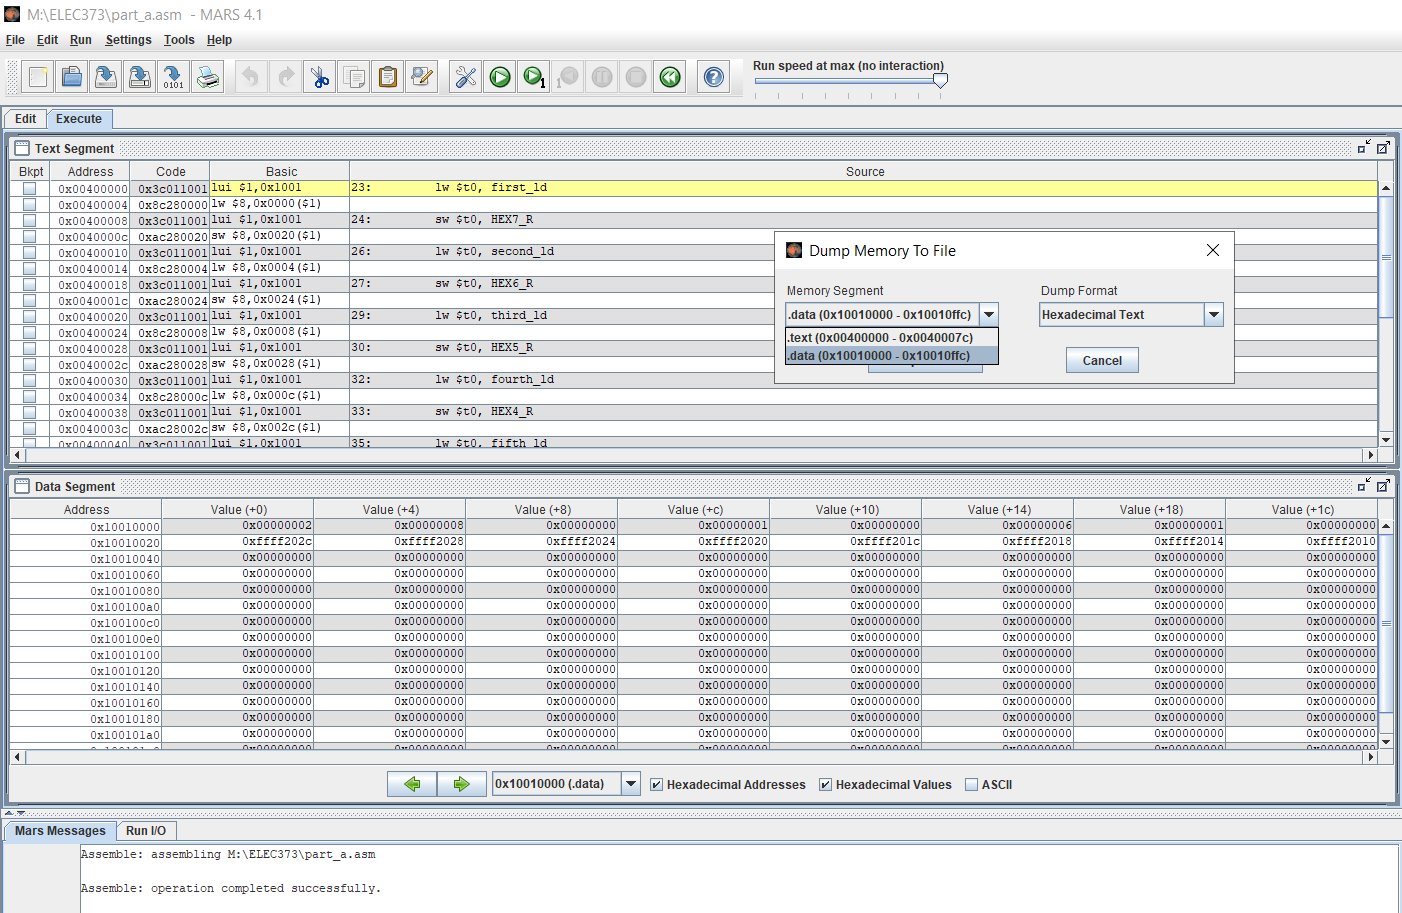
\includegraphics[width=\textwidth]{dump}
   \caption{Dump \textit{.data} section to data segment using the \textit{MARS} editor.}
   \label{fig:dump}
\end{figure}
